\section{Results}\label{sec:results}

\subsection{Sigma Hyperparameter Selection}\label{subsec:sigmaHyperparameterSelectionResults}
Recall that $\sigma_1, \sigma_2, \ldots \sigma_n$ are hyperparameters that must be defined prior to executing the
algorithm.
The grid search exhausts every permutation $P_n^{\sigma_n}$, where:
\begin{equation}
    \label{eq:gridSearchQuerySigma}
    \sigma_n \ \in \ \{1.0e^{-16}, 1.0e^{-15}, \ldots 1.0e^{1}\}
\end{equation}
% 2.22 * 10^-16 is the machine epsilon for double

\begin{figure*}
    \centering{
    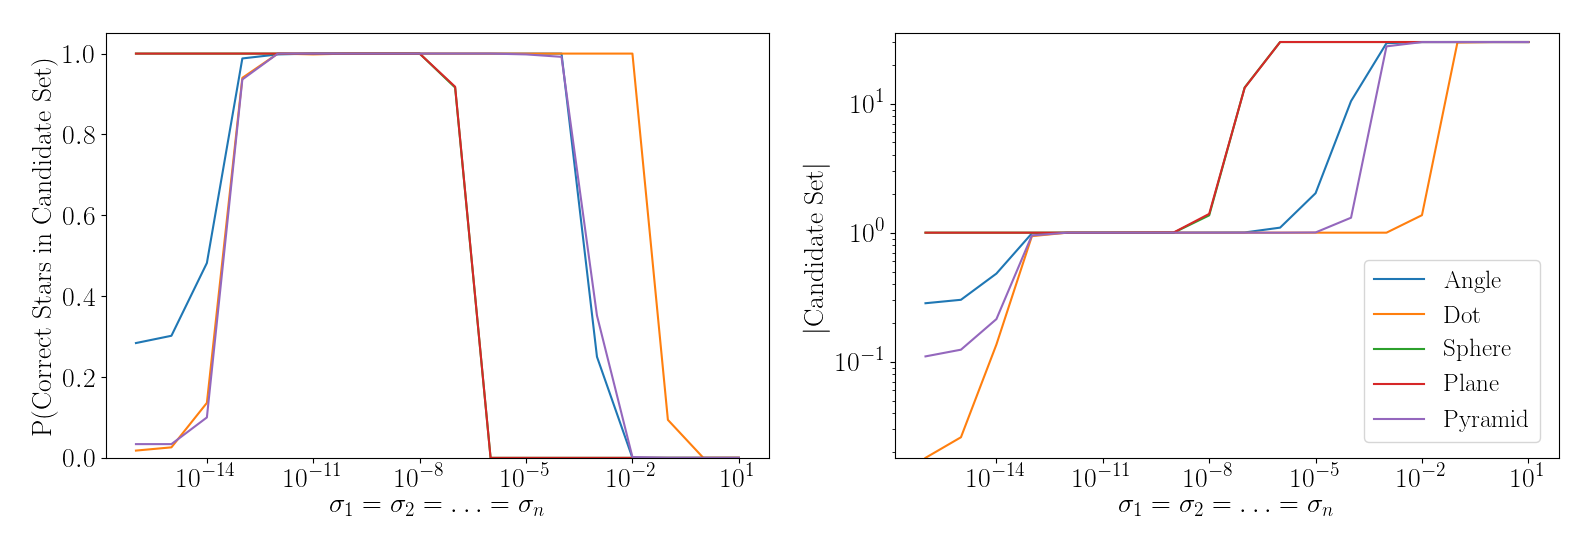
\includegraphics[scale=0.45]{images/sigma1-pcss-css.png}
    \caption{
    The left plot depicts the effect of varying $\sigma$ on the probability that the correct star set exists in the
    resulting candidates after the query.
    The right plot depicts the effect of varying $\sigma$ on the size of the candidate set after the query, bounded
    by 30 candidates at maximum.
    The field-of-view is bounded by $f = 20^\circ$ and the apparent magnitude is bounded by $m = 6.0$.
    Each point represents the average of 100 query steps without noise introduced.
    For brevity, all deviations associated with methods of more than one feature term (i.e.\ Dot Angle, Spherical
    Triangle, \ldots) had all corresponding $\sigma$ terms set equal to each other.
    } \label{figure:sigmaHyperparameterPlots}
    }
\end{figure*}

The set of plots in~\autoref{figure:sigmaHyperparameterPlots} depict the effect on different $\sigma$ terms against the
size of the candidate set $R$ (on the left) and the probability that the correct stars exist in this candidate set (on
the right).
If the deviation is too small, then the selectivity of each query becomes too restrictive and no results are returned.
On the other hand when the selectivity is too high, the candidate set size upper bound of 30 candidates is
hit and the chance that the correct candidate exists in the query declines.

The period of stability for all methods identifying images restricted by $f < 20 \land m < 6.0$ occurs when:
\begin{equation}
    \label{eq:stabilityRegionAcrossFeatures}
    \sigma_n \ \in (10^{-12}, 10^{-8})
\end{equation}
Regardless of the feature, a deviation choice between these bounds should be acceptable for distinguishing stars.

% Not including this, don't feel it is relevant to stability analysis.
%It is important to note that each feature exists in different bounds.
%The values below represent the observed bounds of each feature:
%\begin{alignat*}{2}
%    \label{eq:observedFeatureSpace}
%    % Non-inclusive bounds given below.
%    \theta^{ij} &\in (2.6 \times 10^{-3} &&, 2.0 \times 10^1) \\
%    \theta^{ij} &\in  (2.6 \times 10^{-3} &&, 2.0 \times 10^1) \\
%    \theta^{ic}, \theta^{jc} &\in (2.6 \times 10^{-3} &&, 2.0 \times 10^1) \\
%    \phi &\in (1.3 \times 10^{-3} &&, 1.8 \times 10^2) \\
%    a^{ijk} &\in (3.1 \times 10^{-9} &&, 5.4 \times 10^{-2}) \\
%    \imath^{ijk} &\in (4.8 \times 10^{-16} &&, 5.3 \times 10^{-4}) \\
%    a^{ijk} &\in (3.7 \times 10^{-9} &&, 5.3 \times 10^{-2}) \\
%    \imath^{ijk} &\in (4.9 \times 10^{-16} &&, 5.3 \times 10^{-4})
%\end{alignat*}

\begin{table}
    \centering {
    \caption{
    Query hyperparameter determination stability and sensitivity results of each method.
    The stability length $\ell$ represents the number of deviations where~\autoref{eq:stabilityQuery} is held.
    Each method's critical points $\sigma_{c1}$ and $\sigma_{c2}$ a is the upper bound on the $Q$ and $\lvert R \rvert$
    stability region.
    } \label{tab:sensitivityStabilityResults}
    \begin{tabular}{m{0.27\columnwidth}|m{0.13\columnwidth}|m{0.2\columnwidth}|m{0.2\columnwidth}}
        \textbf{Method} & $\ell$ & $\frac{\partial Q}{\partial\sigma} \text{ at } \sigma_{c1}$ &
        $\frac{\partial \lvert R \rvert}{\partial \sigma} \text{ at } \sigma_{c2}$ \\
        \hline \hline
        \textbf{Angle} & 5 & -0.415 & 0.015 \\ \hline
        \textbf{Dot Angle} & 10 & -0.460 & 0.235 \\ \hline
        \textbf{Spherical \newline Triangle} & 8 & -0.055 & 0.205 \\ \hline
        \textbf{Planar \newline Triangle} & 8 & -0.035 & 0.150 \\ \hline
        \textbf{Pyramid} & 8 & -0.005 & 0.145
    \end{tabular}
    }
\end{table}

Referencing~\autoref{tab:sensitivityStabilityResults}, there appears to some correlation between the number of
\textit{distinct} features and length of the stability region here.
The Dot Angle method uses three total features, two of which are distinct from each other ($\theta$ vs. $\phi$) for
it's query.
The Pyramid method uses three similar features, which has the same stable region length as the triangle methods
using two distinct features.
The Angle method uses only one feature for its query, and suffers in stable region length.

% TODO: How to interpret the Q response?
The largest response belongs to

The candidate set size responses are most likely a result of the size of possible candidates that belong to each
method's respective feature (i.e.\ the number of rows of the table used in query).
The Angle method has the least number of possible candidates given the $f < 20 \land m < 6.0$ constraint, at 353700
possible catalog sets.
The triangle methods have roughly 35 times as many possible catalog sets as the Angle method.
The Dot Angle method has 3 times as many possible catalog sets as the triangle methods, and roughly 105 times as many
possible catalog sets as the Angle method.
Given a larger pool of results to choose from, it follows that the number of false positive increases as well.

The $\sigma$ parameters for the following experiments were chosen using the results of the grid search, and selecting
the largest $\sigma_1, \sigma_2, \sigma_3$ (ordered as such) that maintained all the
conditions in~\autoref{eq:stabilityQuery}.
\begin{alignat*}{2}
    \text{Angle}&: \sigma_\theta &&= 1.0 \times 10^{-4}\\
    \text{Pyramid}&: \sigma_\theta &&= 1.0 \times 10^{-4}\\
    \text{Dot Angle}&: \sigma_{\theta_{ic}} &&= 1.0 \times 10^{-1}\\
    \text{Dot Angle}&: \sigma_{\theta_{jc}} &&= 1.0 \times 10^{-1}\\
    \text{Dot Angle}&: \sigma_\phi &&= 1.0 \times 10^{-3} \\
    \text{Spherical Triangle}&: \sigma_a &&= 1.0 \times 10^{-1}\\
    \text{Spherical Triangle}&: \sigma_\imath &&= 1.0 \times 10^{-11}\\
    \text{Planar Triangle / Composite}&: \sigma_a &&= 1.0 \times 10^{-1} \\
    \text{Planar Triangle / Composite}&: \sigma_\imath &&= 1.0 \times 10^{-11}\\
\end{alignat*}

In addition to the $\sigma_n$ parameters used in the previous experiments, a parameter $\sigma_o$ must be defined
prior to executing the \Call{DMT}{} method.
Each experiment was performed 10 times, and the largest $\sigma_o$ that identification the most stars correctly on
average are displayed below.
These were used for the experiment presented here.
\begin{align*}
    \sigma_o &= 1.0 \times 10^{-4}\\
\end{align*}

\subsection{Query Selectivity}\label{subsec:querySelectivityResults}
Using the optimal hyperparameters described in the previous section, each query step was analyzed in terms of its
response to varying Gaussian noise.

\begin{figure*}
    \centering{
    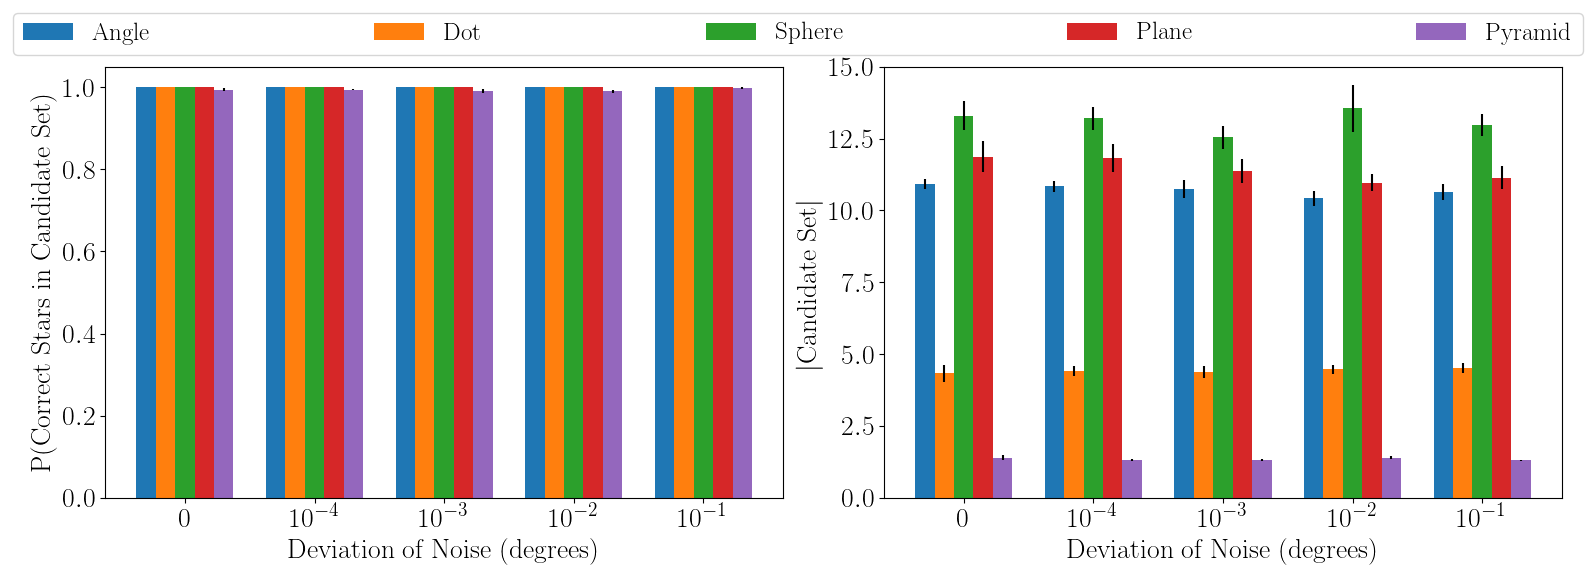
\includegraphics[scale=0.45]{images/query-exp.png}
    \caption{
    The left plot depicts the effect of varying the deviation of Gaussian noise on the probability that the correct
    star set exists in the resulting candidates after the query.
    The right plot depicts the effect of varying this same noise on the size of the candidate set after the query,
    bounded by 5000 candidates at maximum.
    Field of view limit is $f = 20^\circ$.
    Each point represents the average of 5000 query steps.
    For the probability measure these 5000 steps were split into 1000 averages, and the mean of these averages are
    presented above.
    } \label{figure:queryPlots}
    }
\end{figure*}

In~\autoref{figure:queryPlots}, noise is plotted against the probability that the correct stars exist in this
candidate set (on the left) and the size of the candidate set (on the right).
Looking at both graphs, there is no discernible effect of noise on both the probability and the $\lvert R \rvert$ per
method.
This suggests that the \ldots.

On the left, it can be seen that nearly all methods accurate at all levels of noise except for the Pyramid method.
This dips slightly below $P(\text{Correct Stars in } R) = 1$.
On the right, it can be seen that this slight dip in accuracy results in a much smaller $\lvert R \rvert$ size than
the other methods.
The next largest $\lvert R \rvert$ size is seen with the Dot Angle method.

\subsection{Candidate Reduction}\label{subsec:candidateReductionResults}


\subsection{Alignment Determination}\label{subsec:alignmentDeterminationResults}


